\documentclass[tikz,border=12pt]{standalone}
\usepackage{amsmath,amssymb}
\usetikzlibrary{calc,arrows.meta}

\begin{document}
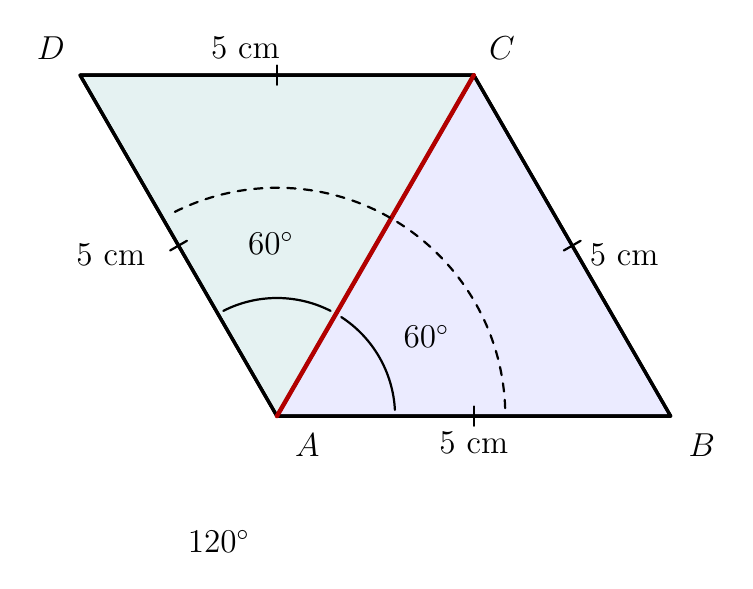
\begin{tikzpicture}[>=latex, line cap=round, line join=round]

  % Rhombus side 5, angle A = 120
  % A=(-2.5,0), B=(2.5,0), AD at 120 deg, length 5: D = (-5, 4.330), C = (0, 4.330)
  \coordinate (A) at (-2.5,0);
  \coordinate (B) at (2.5,0);
  \coordinate (D) at (-5,4.330);
  \coordinate (C) at (0,4.330);

  % shading the two halves
  \draw[very thick, fill=blue!8]  (A) -- (B) -- (C) -- cycle;
  \draw[very thick, fill=teal!10] (A) -- (C) -- (D) -- cycle;
  \draw[very thick] (A) -- (B) -- (C) -- (D) -- cycle;

  % the diagonal AC
  \draw[ultra thick, red!70!black] (A) -- (C);

  % angle work at A
  % outer dashed arc: the whole 120 deg
  \draw[thick, dashed] ($(A) + (2:2.9)$) arc (2:118:2.9);
  \node[font=\large\bfseries] at ($(A) + (245:1.75)$) {$120^\circ$};
  % two inner solid arcs: each 60 deg
  \draw[thick] ($(A) + (3:1.5)$) arc (3:57:1.5);
  \node[font=\large\bfseries] at ($(A) + (28:2.15)$) {$60^\circ$};
  \draw[thick] ($(A) + (63:1.5)$) arc (63:117:1.5);
  \node[font=\large\bfseries] at ($(A) + (92:2.2)$) {$60^\circ$};

  % equal-side ticks (one per side)
  \draw[thick] ($(A)!0.5!(B)!3.5pt!90:(B)$) -- ($(A)!0.5!(B)!3.5pt!270:(B)$);
  \draw[thick] ($(B)!0.5!(C)!3.5pt!90:(C)$) -- ($(B)!0.5!(C)!3.5pt!270:(C)$);
  \draw[thick] ($(C)!0.5!(D)!3.5pt!90:(D)$) -- ($(C)!0.5!(D)!3.5pt!270:(D)$);
  \draw[thick] ($(D)!0.5!(A)!3.5pt!90:(A)$) -- ($(D)!0.5!(A)!3.5pt!270:(A)$);

  % vertex labels
  \node[below right=3pt, font=\large\bfseries] at (A) {$A$};
  \node[below right=3pt, font=\large\bfseries] at (B) {$B$};
  \node[above right=2pt, font=\large\bfseries] at (C) {$C$};
  \node[above left=2pt, font=\large\bfseries] at (D) {$D$};

  % side length labels
  \node[font=\large, below] at (0,-0.08) {$5$ cm};
  \node[font=\large, right] at (1.35,2.05) {$5$ cm};
  \node[font=\large, above] at (-2.9,4.42) {$5$ cm};
  \node[font=\large, left]  at (-4.05,2.05) {$5$ cm};

\end{tikzpicture}
\end{document}
